% !TeX root = ../main.tex

% Edit this title for each week's entry.
\section{Week 8: The Problem with Problematic Observations}

\heading{Module Outline}
\begin{itemize}
    \item Leverage observations
    \item Outlying points in regression
    \item Influential observations
    \item Assessing and addressing problematic observations
\end{itemize}

\begin{remark}[Review: Outliers]
    In previous STA courses, outliers were defined by distance from the median or from
    Q1/Q3: identified visually in a box plot, or numerically with the IQR (beyond
    $Q1-1.5\,IQR$ or $Q3+1.5\,IQR$). Outliers are data points that are, in some way, very far
    from the rest of the data. Statistical outliers are one type of
    \textbf{problematic observation}.
\end{remark}

\begin{definition}[Problematic Observation]
    Any single observation impacting our ability to make accurate inference about the
    parameter(s) (e.g.\ accurate estimation of a mean and variance).
    \begin{itemize}
        \item In regression we estimate many parameters, so many estimates can be impacted by
        one observation: individual coefficients, individual fitted values (conditional mean
        responses, predictions), or the entire regression surface (overall trend).
        \item We need to identify them: do any points have the potential to
        disproportionately impact estimation? How reliable are our estimates?
    \end{itemize}
\end{definition}

\subsection{Leverage Observations}

\begin{center}
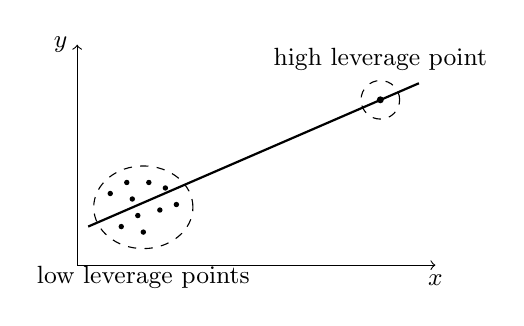
\begin{tikzpicture}[scale=0.7]
    \draw[->] (0,0) -- (6.5,0) node[below]{\small $x$};
    \draw[->] (0,0) -- (0,4) node[left]{\small $y$};
    \draw[thick] (0.2,0.7) -- (6.2,3.3);
    \foreach \p in {(0.6,1.3),(0.8,0.7),(1.0,1.2),(1.1,0.9),(1.3,1.5),(1.5,1.0),(1.6,1.4),(1.8,1.1),(1.2,0.6),(0.9,1.5)}
        \fill \p circle (1.4pt);
    \draw[dashed] (1.2,1.05) ellipse (0.9 and 0.75);
    \node[below] at (1.2,0.15) {\small low leverage points};
    \fill (5.5,3.0) circle (1.8pt);
    \draw[dashed] (5.5,3.0) circle (0.35);
    \node[above] at (5.5,3.35) {\small high leverage point};
\end{tikzpicture}
\end{center}

\begin{definition}[Leverage]
    The leverage of a point measures how far it is from the centre in terms of
    $\mathbf{X}$ (``outliers'' in $\mathbf{X}$ are high leverage).
    \begin{itemize}
        \item [High] leverage points have the \underline{potential} to change the line of best
        fit (be high influence).
        \item A \textbf{leverage observation} is an observation very distant from the centre of
        the $\mathbf{X}$-space that \textbf{may} change $\hat{\mathbf{Y}}$.
        \item In SLR, a leverage point is far from the other points on the horizontal axis.
    \end{itemize}
\end{definition}

\begin{remark}[Concept of Leverage]
    ``Leverage'' comes from ``lever'': the longer the lever, the more weight you can move with
    little effort. \textbf{Fulcrum}: the centre of the predictors $\mathbf{X}$.
    \textbf{Lever}: the regression surface. \textbf{High leverage points}: far from the
    fulcrum. Leverage points have the potential to shift the regression line, but will not
    always do it.
\end{remark}

\begin{definition}[Hat Matrix and Leverage $h_{ii}$]
    Leverage must incorporate (1) the distance between the predictor values and the centre of
    all predictors, and (2) how much the estimated trend \underline{could} change because of
    this observation. Recall the hat matrix $\mathbf{H}=\mathbf{X}(\mathbf{X}'\mathbf{X})^{-1}\mathbf{X}'$,
    which projects $\mathbf{Y}$ onto the model space through $\mathbf{X}$:
    \[\hat{\mathbf{Y}}=\mathbf{X}\hat{\boldsymbol\beta}=\mathbf{X}(\mathbf{X}'\mathbf{X})^{-1}\mathbf{X}'\mathbf{Y}=\mathbf{H}\mathbf{Y},\qquad
    \begin{pmatrix}\hat y_1\\ \vdots\\ \hat y_n\end{pmatrix}=
    \begin{pmatrix}h_{11}&\cdots&h_{1n}\\ \vdots&\ddots&\vdots\\ h_{n1}&\cdots&h_{nn}\end{pmatrix}
    \begin{pmatrix}y_1\\ \vdots\\ y_n\end{pmatrix}\]
    Each fitted value is a linear combination of \emph{all} the $y_j$'s with coefficients $h_{ij}$:
    \[\hat y_i=h_{i1}y_1+\cdots+h_{in}y_n=\hly{h_{ii}y_i}+\sum_{j\neq i}h_{ij}y_j\]
    \begin{itemize}
        \item $h_{ii}$ is the contribution of $y_i$ predicting itself; $h_{ij}$ is the
        contribution of $y_j$ to predicting $\hat y_i$.
        \item The diagonal element \rb{$h_{ii}$ is the leverage of observation $i$}: how much
        impact $y_i$ has on $\hat y_i$ (vs.\ the other $n-1$ $y_j$'s).
        \item High leverage: $\hat y_i$ is dragged towards $y_i$. Low leverage: $\hat y_i$ is
        not really impacted by the value of $y_i$.
    \end{itemize}
\end{definition}

\begin{proposition}[Leverage in SLR]
    \[\boxed{h_{ii}=\frac1n+\frac{(x_i-\bar x)^2}{\sum_{j=1}^n(x_j-\bar x)^2}}\]
    The second term is the ratio of the \textbf{squared distance between $x_i$ and $\bar x$} to
    the \textbf{total variation in the predictor} --- ``how much variability in $X$ does $x_i$
    contribute?''. $h_{ii}$ is minimized at $x_i=\bar x$, and the further $x_i$ is from $\bar x$,
    the higher its leverage.
\end{proposition}

\begin{proposition}[Properties of the Hat Matrix]
    \begin{enumerate}
        \item $\sum_{i=1}^nh_{ii}=p+1$ (the number of $\beta$'s), so the \textbf{average leverage}
        is $(p+1)/n$. Most datasets have $n\gg p$, so most leverages are close to 0.
        \aside{Aside: we typically want $\sim$15--20 observations per $\beta$, as a bare minimum.}
        \item $0\leq h_{ii}\leq1$: leverage is the \emph{fraction} of $\hat y_i$ due to $y_i$
        vs.\ the other responses.
    \end{enumerate}
\end{proposition}

\begin{proof}
    (1) The trace $\mathrm{Tr}$ of a square matrix is the sum of its diagonal, and it is
    invariant under cyclic shifts: $\mathrm{Tr}(\mathbf{ABCD})=\mathrm{Tr}(\mathbf{BCDA})=\mathrm{Tr}(\mathbf{CDAB})=\mathrm{Tr}(\mathbf{DABC})$. So
    \[\sum_{i=1}^nh_{ii}=\mathrm{Tr}(\mathbf{H})=\mathrm{Tr}\big(\mathbf{X}(\mathbf{X}'\mathbf{X})^{-1}\mathbf{X}'\big)
    =\mathrm{Tr}\big(\mathbf{X}'\mathbf{X}(\mathbf{X}'\mathbf{X})^{-1}\big)=\mathrm{Tr}(\mathbf{I}_{p+1})=p+1\]
    (2) $\mathbf{H}$ is idempotent ($\mathbf{H}=\mathbf{H}^2$) and symmetric, so the $i$-th
    diagonal element of $\mathbf{H}^2$ (row $i$ of $\mathbf{H}$ times column $i$ of $\mathbf{H}$) gives
    \[h_{ii}=\sum_{j=1}^nh_{ij}^2=\underbrace{h_{ii}^2}_{\geq0}+\underbrace{\sum_{j\neq i}h_{ij}^2}_{\geq0}
    \ \Rightarrow\ h_{ii}\geq h_{ii}^2\ \Rightarrow\ 0\leq h_{ii}\leq1\qedhere\]
\end{proof}

\begin{remark}[Leverage of Observation $i$]
    \begin{itemize}
        \item $h_{ii}$ tells us how much $\hat y_i$ is driven by $y_i$: how much the regression
        line is \hlt{potentially} dragged towards this one observation because of its distance
        from the centre.
        \item Since most $h_{ii}$ are small, if $h_{ii}\approx1$ then the other $h_{ij}\approx0$
        (usually): observation $i$ is far from the rest of the data, and
        $\hat y_i=h_{ii}y_i+\sum_{j\neq i}h_{ij}y_j\approx y_i$, so the fit was pulled towards $y_i$.
        If the dataset did not contain observation $i$, a different line/surface might have been estimated!
        \item Recall $\Var(\hat{\boldsymbol\epsilon})=\Var\big((\mathbf{I}-\mathbf{H})\mathbf{Y}\big)=\sigma^2(\mathbf{I}-\mathbf{H})$,
        so $\Var(\hat\epsilon_i)=\sigma^2(1-h_{ii})$: residuals of high leverage points are smaller
        in magnitude (have smaller variance).
        \item High leverage does \textbf{not} always mean the line has shifted --- it just has the
        \hlt{potential} to. Some sources (e.g.\ Sheather) call these ``good'' leverage points if
        they don't shift the line and ``bad'' leverage points if they do.
    \end{itemize}
\end{remark}

\begin{example}[Regression Influence Applet ($n=20$, $p=1$)]
    All 20 points give $\hat y=15.1854-0.5185x$ (SSE $347.279$). Removing one point at a time:
    \begin{center}
        \begin{tabular}{lrrr}
            \toprule
            Point removed & Intercept & Slope & SSE \\
            \midrule
            none (all data) & 15.1854 & $-0.5185$ & 347.279 \\
            high $y$, middle $x\approx10$ \aside{(low leverage)} & 14.5467 & $-0.5184$ & 193.090 \\
            far right, $x\approx20$ \aside{(high leverage)} & 14.2514 & $-0.3965$ & 323.237 \\
            far left, $x\approx-2$ \aside{(high leverage)} & 15.3933 & $-0.5359$ & 346.974 \\
            \bottomrule
        \end{tabular}
    \end{center}
    \db{The low leverage point barely changes the line (only shifts it slightly) even with a
    huge residual. The far-right high leverage point changes the slope noticeably; the far-left
    one lies near the line, so removing it changes little.}
\end{example}

\begin{definition}[Identifying Leverage Points]
    $(\mathbf{x}_i,y_i)$ has high leverage if
    \begin{itemize}
        \item $h_{ii}>\frac{2(p+1)}{n}$ (Hoaglin and Welsch, 1978);
        \item $h_{ii}>\frac{3(p+1)}{n}$ for $p>6$ and $n-p>12$ (Velleman and Welsch, 1981);
        \item $h_{ii}>0.5$ (Huber, 1981).
    \end{itemize}
    \textbf{In this class}: \[\boxed{h_{ii}>\frac{2(p+1)}{n}}\quad\text{(more than twice the average leverage)}\]
\end{definition}

\subsection{Outlying Points in Regression}

\begin{definition}[Outlier in Regression]
    A data point that the model fails to explain: far away from the trend, i.e.\ with a
    \textbf{large residual}.
    \[\hat{\mathbf{Y}}=\mathbf{H}\mathbf{Y},\qquad \hat{\mathbf{e}}=\mathbf{Y}-\hat{\mathbf{Y}}=(\mathbf{I}-\mathbf{H})\mathbf{Y}\]
    Residuals are the observed responses weighted by $\mathbf{I}-\mathbf{H}$ (the ``residual
    maker'' or ``annihilator'' matrix), so we can use them to measure each observation's
    potential to attract the regression line.
\end{definition}

\begin{proposition}[Leverage and Residuals]
    Writing $\hat{\mathbf{e}}=(\mathbf{I}-\mathbf{H})\mathbf{Y}$ out row by row,
    \[\hat e_i=-h_{i1}y_1-\cdots+(1-h_{ii})y_i-\cdots-h_{in}y_n=\underline{(1-h_{ii})y_i}-\sum_{j\neq i}h_{ij}y_j\]
    \aside{Equivalently $\hat e_i=y_i-\hat y_i=y_i-\big(h_{ii}y_i+\sum_{j\neq i}h_{ij}y_j\big)$.}
    Since $0\leq h_{ii}\leq1$, the impact of $y_i$ on $\hat e_i$ depends on its leverage:
    \begin{itemize}
        \item the higher the leverage, the lower the weight this observation has on its residual;
        \item high leverage observations have smaller (in magnitude) residuals, since the fit is
        dragged towards them.
    \end{itemize}
    Recall (Modules 3 \& 5):
    $\Cov(\hat{\mathbf{e}}\mid\mathbf{X})=(\mathbf{I}-\mathbf{H})\sigma^2(\mathbf{I}-\mathbf{H})'=\sigma^2(\mathbf{I}-\mathbf{H})$,
    so the residuals do \textbf{not} have constant variance: $\Var(\hat e_i\mid\mathbf{X})=\sigma^2(1-h_{ii})$.
\end{proposition}

\begin{definition}[Standardized Residuals]
    We want residuals with the same properties as the errors (for checking assumptions,
    etc.), so standardize each $\hat e_i$ by its standard error:
    \[\boxed{r_i=\frac{\hat e_i}{s\sqrt{1-h_{ii}}}}\]
    \begin{itemize}
        \item $r_i$ have constant variance.
        \item $r_i$ combines the \textbf{residual value} ($\hat e_i$), the \textbf{leverage}
        ($h_{ii}$) and the \textbf{estimated error variance} ($s$).
        \item $r_i$ more fairly measures ``outlying-ness'' by adjusting for leverage, and tells us
        \textbf{how many standard deviations away from the estimated trend} the observation is.
        \item Useful for checking assumptions, especially with high leverage points: violations
        tend to be more prominent and impactful in the tails (extreme events, remote
        observations) but harder to detect with regular residuals. You don't lose anything by
        using them when there are no high leverage points.
    \end{itemize}
\end{definition}

\begin{definition}[Detecting Outliers (This Class)]
    $(\mathbf{x}_i,y_i)$ is an outlier if
    \[\boxed{r_i\notin[-2,2]\text{ if the dataset is ``small'' (e.g.\ }n<50\text{)},\qquad r_i\notin[-4,4]\text{ if ``large'' (e.g.\ }n\geq50\text{)}}\]
    i.e.\ not within 2 (resp.\ 4) standard deviations. These cutoffs are just a guideline.
    \aside{Recall: one of our model assumptions is that the errors are iid normal.}
\end{definition}

\begin{definition}[Good and Bad Leverage Points]
    Outliers and leverage points are different kinds of problematic observations; both have
    the \underline{potential} to change the estimated regression relationship.
    \begin{itemize}
        \item \textbf{Leverage point}: a data point whose $x$ value is far from the centre.
        \aside{``Depending on the value of $y_i$, this observation has the potential to change
        the line of best fit.''}
        \item \textbf{``Good'' leverage point}: a leverage point that is \emph{not} an outlier.
        \item \textbf{``Bad'' leverage point}: a leverage point that is \emph{also} an outlier.
    \end{itemize}
\end{definition}

\begin{remark}[Sheather Figures 3.4--3.6]
    \begin{itemize}
        \item \textbf{Good leverage point} (Fig.\ 3.4): far from $\bar x$ but very close to the
        line; the least squares line $\hat y=\hat\beta_0+\hat\beta_1x$ stays close to the population line.
        \item \textbf{Bad leverage point} (Fig.\ 3.5): the same point with only its $y$ value
        changed --- now an outlier \emph{and} a leverage point, with a large $\hat e_i$. The least
        squares line is pulled far from the (unobserved) population regression line.
        \item \textbf{Outlier that is not a leverage point} (Fig.\ 3.6): large $\hat e_i$ but $x$
        near the centre, so the line barely moves.
    \end{itemize}
\end{remark}

\begin{example}[Good Leverage, Bad Leverage, or Neither?]
    \begin{center}
    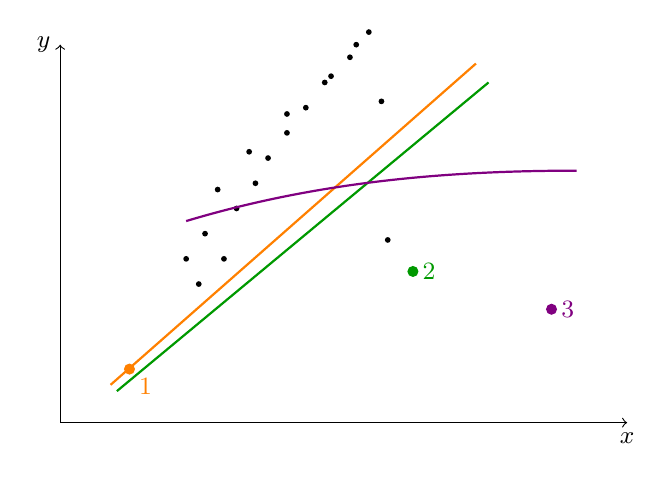
\begin{tikzpicture}[scale=0.8]
        \draw[->] (0,0) -- (9,0) node[below]{\small $x$};
        \draw[->] (0,0) -- (0,6) node[left]{\small $y$};
        \foreach \x/\y in {2.2,2.0/2.6,2.6,2.3/3.0,2.8/3.4,3.1/3.8,3.3/4.2,3.6/4.6,3.9/5.0,4.2/5.4,4.6/5.8,4.9/6.2,5.2/2.9,2.5/3.7,3.0/4.3,3.6/4.9,4.3/5.5,4.7/6.0,5.1}
            \fill (\x,\y) circle (1.3pt);
        \draw[thick,orange] (0.8,0.6) -- (6.6,5.7);
        \draw[thick,green!60!black] (0.9,0.5) -- (6.8,5.4);
        \draw[thick,violet] (2.0,3.2) .. controls (4,3.8) and (6,4.0) .. (8.2,4.0);
        \fill[orange] (1.1,0.85) circle (2.5pt) node[below right]{\small 1};
        \fill[green!60!black] (5.6,2.4) circle (2.5pt) node[right]{\small 2};
        \fill[violet] (7.8,1.8) circle (2.5pt) node[right]{\small 3};
    \end{tikzpicture}
    \end{center}
    \begin{itemize}
        \item \db{\textbf{Point 1}: leverage point, not an outlier, not influential
        $\Rightarrow$ \dbb{``good leverage point''}.}
        \item \db{\textbf{Point 2}: not high leverage, outlier, not influential.}
        \item \db{\textbf{Point 3}: outlier, leverage point, influential (drags the fit, as in the
        curved line) $\Rightarrow$ \dbb{``bad leverage point''}.}
    \end{itemize}
\end{example}

\begin{exercise}[Try at Home]
    Using \texttt{mtcars}, fit \texttt{mpg \textasciitilde{} wt + hp + disp}. Compute the
    residuals and leverages (find $\mathbf{H}$ by matrix multiplication, then check with
    \texttt{hatvalues()}). Identify the leverage points --- are they also outliers? What kinds
    of cars are they? Repeat with \texttt{iris}:
    \texttt{Petal.Length \textasciitilde{} Sepal.Length + Sepal.Width + Petal.Width}.
\end{exercise}

\subsection{Influential Observations}

\begin{definition}[Influential Point]
    A data point that \textbf{significantly affects the fitted model}: the regression estimates
    change considerably when it is included vs.\ removed.
    \begin{itemize}
        \item A point can be influential, an outlier, neither, or both. Influential points are not
        necessarily outliers, and outliers are not necessarily influential.
        \item In SLR: plot the regression line with and without the point. If the line changes
        considerably, the point is influential.
    \end{itemize}
\end{definition}

\begin{example}[Three Pictures]
    \begin{itemize}
        \item \textbf{Outlier at the centre} ($x=3$, $y=0$, other points around $y\approx4$): large
        $\hat e_i$, but the LS line with and without it is nearly the same $\Rightarrow$
        \dbb{outlier, not a leverage point, not influential}.
        \item \textbf{Far right, far below} ($x=12$, $y=0$; others in $x\in[0,5]$): the fit goes
        from a clear positive slope to nearly flat --- \dbb{change in estimated slope and
        intercept}; large $\hat e_i$ $\Rightarrow$ \dbb{influential}.
        \item \textbf{Very far right, near the trend's extension} ($x=50$, $y=20$; others in
        $x\in[0,6]$): \dbb{very high leverage}; small $\hat e_i$ (because the line is dragged to
        it) so unsure if it's an outlier, but the slope and intercept change $\Rightarrow$
        \dbb{influential}.
    \end{itemize}
\end{example}

\begin{remark}[Quantifying Influence in MLR]
    A problematic $(\mathbf{x}_i,y_i)$ can influence the estimates of
    \begin{itemize}
        \item all fitted values $\hat{\mathbf{Y}}$ $\to$ \textbf{Cook's distance};
        \item its own fitted value $\hat y_i$ $\to$ \textbf{DFFITS};
        \item the trend, i.e.\ at least one coefficient $\hat{\boldsymbol\beta}$ $\to$ \textbf{DFBETAS}.
    \end{itemize}
    All three are \textbf{``delete-one'' measures}: does the model change a lot after deleting
    the $i$-th observation, or mostly stay the same? A subscript $(i)$ denotes values from the
    model fit with the $i$-th observation deleted (using the other $n-1$).
\end{remark}

\begin{definition}[Cook's Distance (Influence on All Fitted Values)]
    Fit the model with all $n$ observations, refit with observation $i$ removed, and compare
    the fitted values (or, equivalently, the coefficients):
    \[\boxed{D_i=\frac{(\hat{\mathbf{Y}}_{(i)}-\hat{\mathbf{Y}})'(\hat{\mathbf{Y}}_{(i)}-\hat{\mathbf{Y}})}{(p+1)s^2}}
    =\frac{(\hat{\boldsymbol\beta}_{(i)}-\hat{\boldsymbol\beta})'\mathbf{X}'\mathbf{X}(\hat{\boldsymbol\beta}_{(i)}-\hat{\boldsymbol\beta})}{(p+1)s^2}\]
    With $(\hat{\mathbf{Y}}_{(i)}-\hat{\mathbf{Y}})'(\hat{\mathbf{Y}}_{(i)}-\hat{\mathbf{Y}})=\sum_{j=1}^n(\hat y_{(i),j}-\hat y_j)^2$
    and $s^2=\frac{RSS}{n-p-1}$,
    \[D_i=\frac{\sum_{j=1}^n(\hat y_{(i),j}-\hat y_j)^2/(p+1)}{RSS/(n-p-1)},\]
    a ratio of mean squares.
\end{definition}

\begin{proposition}[Cook's Distance --- Simplified Form]
    Instead of fitting $n$ delete-one models, using only the full model:
    \[\boxed{D_i=\underbrace{\frac{r_i^2}{p+1}}_{\text{outlying-ness}}\ \underbrace{\frac{h_{ii}}{1-h_{ii}}}_{\text{leverage}}}\]
    Cook's D incorporates being far from the centre in $X$ (leverage; $\frac{h_{ii}}{1-h_{ii}}$
    is sometimes called the ``\textbf{potential}'') and being far from the estimated trend in $Y$
    (outlying-ness, via the residual).
\end{proposition}

\begin{definition}[Influential by Cook's Distance]
    Influential points have high $D_i$ compared to the other points. Guideline (Cook, 1977):
    observation $i$ is influential if
    \[\boxed{D_i>F_{0.5}(p+1,\,n-p-1)}\quad\text{(the \textbf{median of $F(p+1,n-p-1)$})}\]
    \aside{Other authors use a cutoff of 1 or $4/n$; this course uses $F_{0.5}(p+1,n-p-1)$.}
\end{definition}

\begin{definition}[DFFITS (Influence on Its Own Fitted Value)]
    ``DiFference in FITted values, Standardized'': the change in $\hat y_i$ when observation $i$
    is removed, accounting for the variation expected. Less conservative than Cook's distance.
    \[\boxed{DFFITS_i=\frac{\hat y_i-\hat y_{i(i)}}{\sqrt{s_{(i)}^2h_{ii}}}}\]
    \begin{itemize}
        \item $\hat y_i$ is the fitted value; $\hat y_{i(i)}$ is the \textbf{prediction} for
        observation $i$ from the model without $i$.
        \item $s_{(i)}^2$ is the estimated error variance from the model without $i$.
    \end{itemize}
    Like Cook's D, it can be computed from the full model:
    \[DFFITS_i=\underbrace{\Big(\frac{h_{ii}}{1-h_{ii}}\Big)^{0.5}}_{\text{leverage}}\underbrace{\frac{\hat e_i}{s_{(i)}\sqrt{1-h_{ii}}}}_{\text{outlying-ness}}\]
    \aside{The second factor is almost $r_i$ (with $s_{(i)}$ instead of $s$).}
    \\ Rule of thumb: examine observation $i$ more closely if
    \[\boxed{|DFFITS_i|>2\sqrt{(p+1)/n}}\]
\end{definition}

\begin{definition}[DFBETAS (Influence on at Least One Coefficient)]
    ``DiFference in BETAs, Standardized'': delete each of the $n$ observations individually and
    compare each of the $p+1$ coefficients individually, so there are $n\times(p+1)$ DFBETAS.
    Compare the change in $\hat\beta_j$ to the expected variation from its sampling distribution:
    \[\boxed{DFBETAS_{j(i)}=\frac{\hat\beta_j-\hat\beta_{j(i)}}{\sqrt{s_{(i)}^2(\mathbf{X}'\mathbf{X})^{-1}_{j+1,j+1}}}}\]
    \begin{itemize}
        \item $\hat\beta_{j(i)}$: coefficient $j$ from the model without point $i$; $s_{(i)}^2$:
        error variance estimate from the model without $i$.
        \item $(\mathbf{X}'\mathbf{X})^{-1}_{j+1,j+1}$: the $(j+1)$-th diagonal element of
        $(\mathbf{X}'\mathbf{X})^{-1}$ computed with \emph{all} observations.
        \aside{Since $\Var(\hat{\boldsymbol\beta})=\sigma^2(\mathbf{X}'\mathbf{X})^{-1}$ is estimated by
        $s^2(\mathbf{X}'\mathbf{X})^{-1}$, $\widehat{\Var}(\hat\beta_j)=s^2(\mathbf{X}'\mathbf{X})^{-1}_{j+1,j+1}$.}
        \item Unlike the others, it does not simplify.
    \end{itemize}
    Rule of thumb for the course: examine observation $i$ more closely if
    \[\boxed{|DFBETAS_{j(i)}|>2/\sqrt n}\text{ for some }j\]
\end{definition}

\begin{remark}[Influence Measures]
    To decide whether a case is influential, compare the fitted model with and without it and
    examine the impact on parameter estimates or predictions. Identifying influential
    observations is \textbf{subjective} --- neither automatic nor foolproof. Cook's distance,
    DFFITS and DFBETAS all assess the impact of removing a single observation, similar to
    leave-one-out cross-validation (LOOCV; Module 10).
\end{remark}

\subsection{Assessing and Addressing Problematic Observations}

\begin{remark}[Problematic Observations]
    \begin{itemize}
        \item Points that can \emph{potentially} influence the trend: leverage points and
        outliers. Points that \emph{do} influence some aspect of the trend: influential points.
        \item Always check leverage, outliers and all 3 influence measures for every observation:
        we need to understand why the fitted surface is the way it is, and some points are flagged
        by one measure but not others.
        \item Identify problematic observations \textbf{both before and after model selection}.
    \end{itemize}
\end{remark}

\begin{center}
    \begin{tabular}{lll}
        \toprule
        Type of point & Measure & Cutoff for this class \\
        \midrule
        Leverage & $h_{ii}$ & $h_{ii}>2\,\frac{p+1}{n}$ \\[3pt]
        Outlier & $r_i$ & $r_i\notin[-2,2]$ if ``small'' ($n<50$); $r_i\notin[-4,4]$ if ``large'' ($n\geq50$) \\[3pt]
        Influence & $D_i$ & $D_i>F_{0.5}(p+1,\,n-p-1)$ \\
        & $DFFITS_i$ & $|DFFITS_i|>2\sqrt{(p+1)/n}$ \\
        & $DFBETAS_{j(i)}$ & $|DFBETAS_{j(i)}|>2/\sqrt n$ \\
        \bottomrule
    \end{tabular}
    \\[2pt] \textit{\small Summary of cutoffs for identifying problematic observations.}
\end{center}

\begin{example}[Bonds Pricing Data (Sheather p.\ 61)]
    From the Nov 9, 1988 \emph{Wall Street Journal}: Coupon Rate ($X$, the fixed interest
    payment on a bond) vs.\ Bid Price ($Y$, what a buyer is willing to pay) for 35 bonds. Cases
    \#4, \#13 and \#35 sit at low coupon rates ($\approx3$--$4\%$) with bid prices $\approx95$, well
    above the trend of the rest, and look potentially highly influential. Sheather's diagnostics
    for case 13: coupon rate 3.000, bid price 94.50, leverage 0.218, residual 10.515,
    standardized residual 2.848 --- the highest Cook's distance and the largest standardized
    residual. \aside{Sheather's Cook's distance plot uses a different cutoff from ours.}
\begin{verbatim}
data <- read.table("bonds.txt", header=T)
bondsModel       <- lm(BidPrice ~ CouponRate, data=data)        # all obs
bondsModel_del13 <- lm(BidPrice ~ CouponRate, data=data[-13,])  # obs 13 removed
n = 35
p = 1
\end{verbatim}
\end{example}

\begin{example}[Bonds: Case 13 ``Manually'']
    Intermediate values: $s_x^2=5.45$, $\bar x=8.92$, $x_{13}=3$, $y_{13}=94.50$,
    $\hat e_{13}=10.5$, $s=4.175$, $s_{(13)}=3.683$.
\begin{verbatim}
sx     <- var(data$CouponRate)
xbar   <- mean(data$CouponRate)
x13    <- data$CouponRate[13]
y13    <- data$BidPrice[13]
e13    <- y13 - bondsModel$fitted.values[13]
s      <- sqrt(sum((bondsModel$residuals)^2)/(n-p-1))
s_del13 <- sqrt(sum((bondsModel_del13$residuals)^2)/(n-1-p-1))
# denominator for s_del13 has 1 less because obs #13 is deleted
\end{verbatim}
    \begin{enumerate}
        \item \textbf{Leverage}:
        \[h_{13}=\frac1n+\frac{(x_{13}-\bar x)^2}{(n-1)s_x^2}=\frac1{35}+\frac{(3-8.92)^2}{34(5.45)}=0.218>2\Big(\frac{2}{35}\Big)=0.11\]
        $\Rightarrow$ \dbb{high leverage point}.
        \item \textbf{Standardized residual}:
        \[r_{13}=\frac{\hat e_{13}}{s\sqrt{1-h_{13}}}=\frac{94.5-83.98}{4.175\sqrt{1-0.218}}=2.85>2\]
        $\Rightarrow$ \dbb{outlier}. So case 13 is a high leverage point that is also an outlier:
        a \dbb{bad leverage point}.
        \item \textbf{Cook's distance}:
        \[D_{13}=\frac{r_{13}^2}{p+1}\,\frac{h_{13}}{1-h_{13}}=\frac{2.85^2}{2}\times\frac{0.218}{1-0.218}=1.13\]
        Cutoff: \texttt{qf(0.5, p+1, n-p-1)} $=$ \texttt{qf(0.5, 2, 33)} $=0.71$
        \aside{(median, $df_1$, $df_2$)} $\Rightarrow$ \dbb{influential}.
        \item \textbf{DFFITS}:
        \[DFFITS_{13}=\Big(\frac{0.218}{1-0.218}\Big)^{0.5}\frac{94.5-83.98}{3.683\sqrt{1-0.218}}=1.70>2\sqrt{2/35}=0.48\]
        $\Rightarrow$ \dbb{influential on its own fitted value}.
        \item \textbf{DFBETAS} (slope), with $(\mathbf{X}'\mathbf{X})^{-1}_{2,2}=0.0054$:
        \[DFBETAS_{1(13)}=\frac{\hat\beta_1-\hat\beta_{1(13)}}{s_{(13)}\sqrt{(\mathbf{X}'\mathbf{X})^{-1}_{2,2}}}=\frac{3.07-3.50}{3.683\sqrt{0.0054}}=-1.59,\quad|{-1.59}|>2/\sqrt{35}=0.34\]
        $\Rightarrow$ \dbb{influential on the estimated slope} \aside{(repeat for $\hat\beta_0$ if
        interested in the intercept)}.
    \end{enumerate}
\begin{verbatim}
h13 <- 1/n + (x13 - xbar)^2/((n-1)*sx)         # 0.2178763
r13 <- e13/(s*sqrt(1-h13))                     # 2.847548
D13 <- r13^2/(p+1)*h13/(1-h13)                 # 1.129397
DFFITS13 <- sqrt(h13/(1-h13))*e13/(s_del13*sqrt(1-h13))   # 1.704072
X <- model.matrix(bondsModel)
XtXinv_22 <- solve(t(X) %*% X)[2,2]            # 0.005398943
(bondsModel$coefficients[2] - bondsModel_del13$coefficients[2]) /
  (s_del13*sqrt(XtXinv_22))                    # -1.588415
cutoff_di     <- qf(0.5, p+1, n-p-1)
cutoff_dffits <- 2*sqrt((p+1)/n)
cutoff_dfbetas <- 2/sqrt(n)        # 0.7079124 0.4780914 0.3380617
\end{verbatim}
\end{example}

\heading{Useful R Functions}
\begin{itemize}
    \item \texttt{rstandard()} --- standardized residuals
    \item \texttt{hatvalues()} --- leverage values
    \item \texttt{cooks.distance()}, \texttt{dffits()}, \texttt{dfbetas()} --- the three influence measures
    \item \texttt{influence.measures()} --- all of the above and more (see its help file)
\end{itemize}

\begin{example}[Bonds Using R]
    Pass the fitted model object to each function, and use \texttt{which()} to check the cutoffs:
\begin{verbatim}
hii <- hatvalues(bondsModel);      hii[13]      # 0.2178763
ri  <- rstandard(bondsModel)
which(ri > 2 | ri < -2)                         # 13 34 35  (| is OR)
ri[13]                                          # 2.847548
dffits(bondsModel)[13]                          # 1.704072
dfbetas(bondsModel)[13,]   # (Intercept) 1.692184, CouponRate -1.588415
cooks.distance(bondsModel)[13]                  # 1.129397
\end{verbatim}
    \aside{\texttt{which()} prints both the row number and row name (the same here). The
    \texttt{dfbetas()} columns are $\beta_0$ and $\beta_1$.}
\end{example}

\begin{exercise}[Try at Home: \texttt{mtcars}]
    Fit the SLR \texttt{mpg \textasciitilde{} hp}, plot \texttt{mpg} vs.\ \texttt{hp} with the line of
    best fit, and find $D_i$, $DFFITS_i$ and $DFBETAS$ for each point, flagging influential ones
    with the cutoffs. Mark them on the scatterplot: what do you see, and what happens when you
    remove them? Is there a pattern in the kinds of cars?
\begin{verbatim}
n = 32; p = 1
model_mtcars <- lm(mpg ~ hp, data = mtcars)
plot(mtcars$hp, mtcars$mpg); abline(model_mtcars, col = "red")
influence.measures(model_mtcars)
cooks.distance(model_mtcars) > qf(0.5, p+1, n-p-1)
dffits(model_mtcars)  > 2*sqrt((p+1)/n)
dfbetas(model_mtcars) > 2/sqrt(n)
\end{verbatim}
    \db{The Maserati Bora (hp $\approx335$, far right) is flagged. Options: justify removing
    \emph{all} sports cars; add a predictor for kind of car, country of origin, etc.; or do
    nothing and discuss the limitations.}
\end{exercise}

\begin{remark}[Addressing Problematic Observations]
    Three approaches for influential observations:
    \begin{enumerate}
        \item \textbf{Consider removing them \underline{only if justified}} (e.g.\ invalid observations).
        \begin{itemize}
            \item \textbf{Do not} remove observations just to improve the model --- this is like p-hacking.
            \item Typically, note the presence of problematic points (be transparent) and their
            impact as a limitation of the model.
            \item If a point is deleted, say so clearly; it \textbf{must} be justified. Removal
            should be the last option.
        \end{itemize}
        \item \textbf{Modify the model} (e.g.\ transform variables or add interaction terms).
        \item \textbf{Use alternative estimation methods} (e.g.\ robust regression or weighted
        least squares, in later STA courses).
    \end{enumerate}
\end{remark}

\begin{example}[Discussion: Tiger Woods]
    In the golfing dataset (MarkUs worksheet), a highly problematic observation is Tiger Woods
    --- an exceptionally good player. Arguments for and against removing it?
    \\\db{Add a predictor (e.g.\ which league they're in) to differentiate players more; or
    remove \emph{all} pro players and focus the analysis on amateurs.}
\end{example}

\begin{remark}[Summary]
    \begin{itemize}
        \item Leverage points and outliers are potentially problematic and may be influential;
        leverage points are not necessarily outliers, and vice versa.
        \item Use leverage $h_{ii}$ to identify leverage points (unusual in predictor space).
        \item Use standardized (or studentized) residuals to detect outliers.
        \item Use Cook's distance, DFFITS and DFBETAS to assess influence on the estimates.
    \end{itemize}
    \aside{Next week: model selection tools and methods --- which predictors do we include, and
    how do we decide?}
\end{remark}
